\subsection{Per-question correlation and paradigm complementarity}
\label{sec:results-correlation}

The pass@k results compare aggregate accuracies. Per-question accuracy vectors carry a finer signal: for each model, the fraction of $n$ samples that solve a given question. Pearson correlations between these vectors quantify how strongly two models share failure modes. Figure~\ref{fig:correlation-summary} and Table~\ref{tab:corr-summary} report the within-paradigm and strongest cross-paradigm correlation for each of the six main conditions; the full pairwise matrices are reproduced in Appendix~\ref{sec:appendix-correlation}.

\begin{figure}[!htbp]
\centering
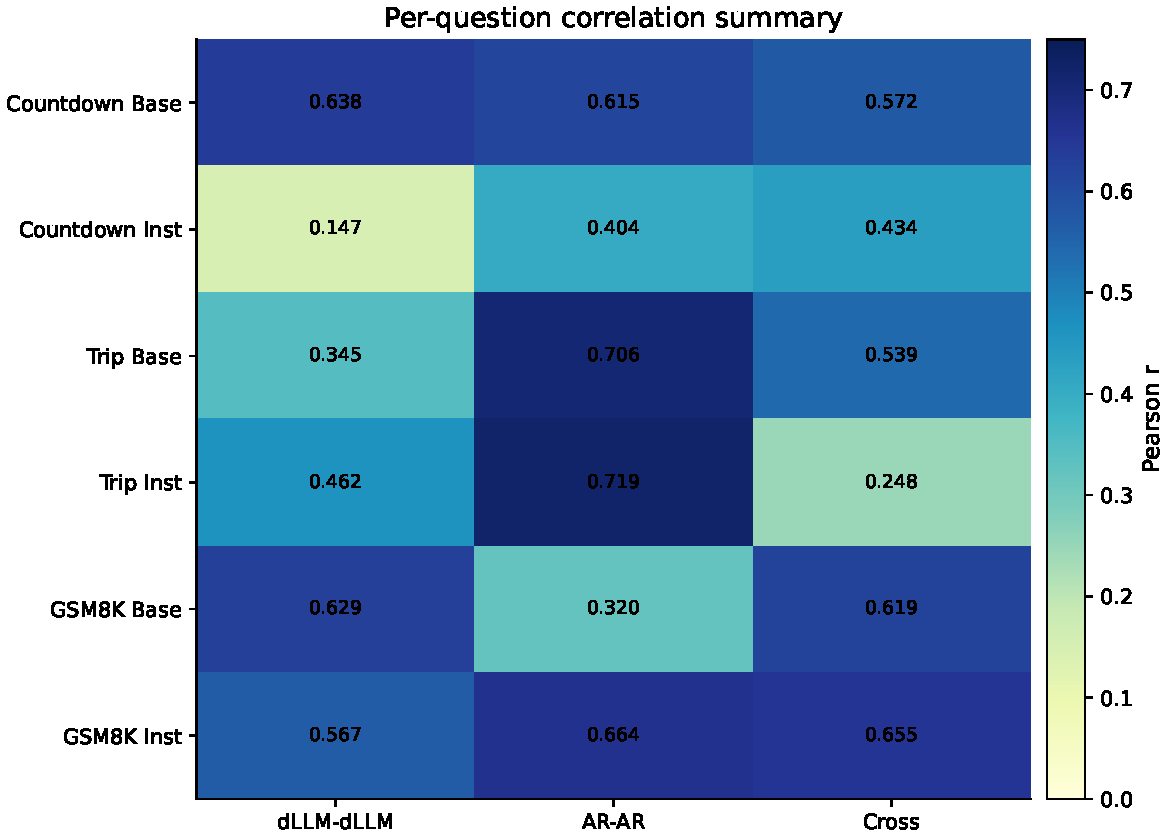
\includegraphics[width=0.84\textwidth]{images/correlation_summary.pdf}
\caption{Within-paradigm and strongest cross-paradigm Pearson correlations across the six main comparison conditions. Countdown Base has the strongest dLLM--dLLM agreement, while Trip Planning has the strongest AR--AR agreement.}
\label{fig:correlation-summary}
\end{figure}

\begin{table}[!htbp]
\centering
\caption{Within-paradigm and strongest cross-paradigm correlations.}
\label{tab:corr-summary}
\scriptsize
\setlength{\tabcolsep}{4pt}
\begin{tabularx}{\textwidth}{L{2.4cm}cccY}
\toprule
\textbf{Condition} & \textbf{dLLM--dLLM} & \textbf{AR--AR} & \textbf{Cross} & \textbf{Interpretation} \\
\midrule
Countdown Base & $0.638$ & $0.615$ & $0.572$ & Diffusion pair exceeds Dream--Qwen despite Dream's Qwen lineage. \\
Countdown Instruct & $0.148$ & $0.404$ & $0.435$ & LLaDA-Instruct is an outlier; Dream aligns more with AR models. \\
GSM8K Base & $0.629$ & $0.320$ & $0.619$ & Saturated but still shows strong diffusion-pair agreement. \\
GSM8K Instruct & $0.567$ & $0.664$ & $0.655$ & Instruct prompting makes alignments more mixed. \\
Trip Planning Base & $0.345$ & $0.706$ & $0.539$ & AR models share the strongest planning-failure pattern. \\
Trip Planning Instruct & $0.462$ & $0.719$ & $0.248$ & Low cross-paradigm correlations suggest complementarity. \\
\bottomrule
\end{tabularx}
\end{table}

The key result is Countdown Base. LLaDA-Base and Dream-Base correlate at $r=0.638$, which exceeds Dream-Base--Qwen-Base at $r=0.572$ even though Dream shares Qwen's pretrained lineage. For this constrained planning task, generation paradigm is therefore a stronger predictor of failure-mode alignment than shared pretrained architecture. Trip Planning Instruct adds a complementary insight: cross-paradigm correlations are uniformly low, especially Dream-Instruct--Qwen-Instruct at $r=0.157$, which points to complementarity rather than redundancy between the paradigms.

\begin{figure}[!htbp]
\centering
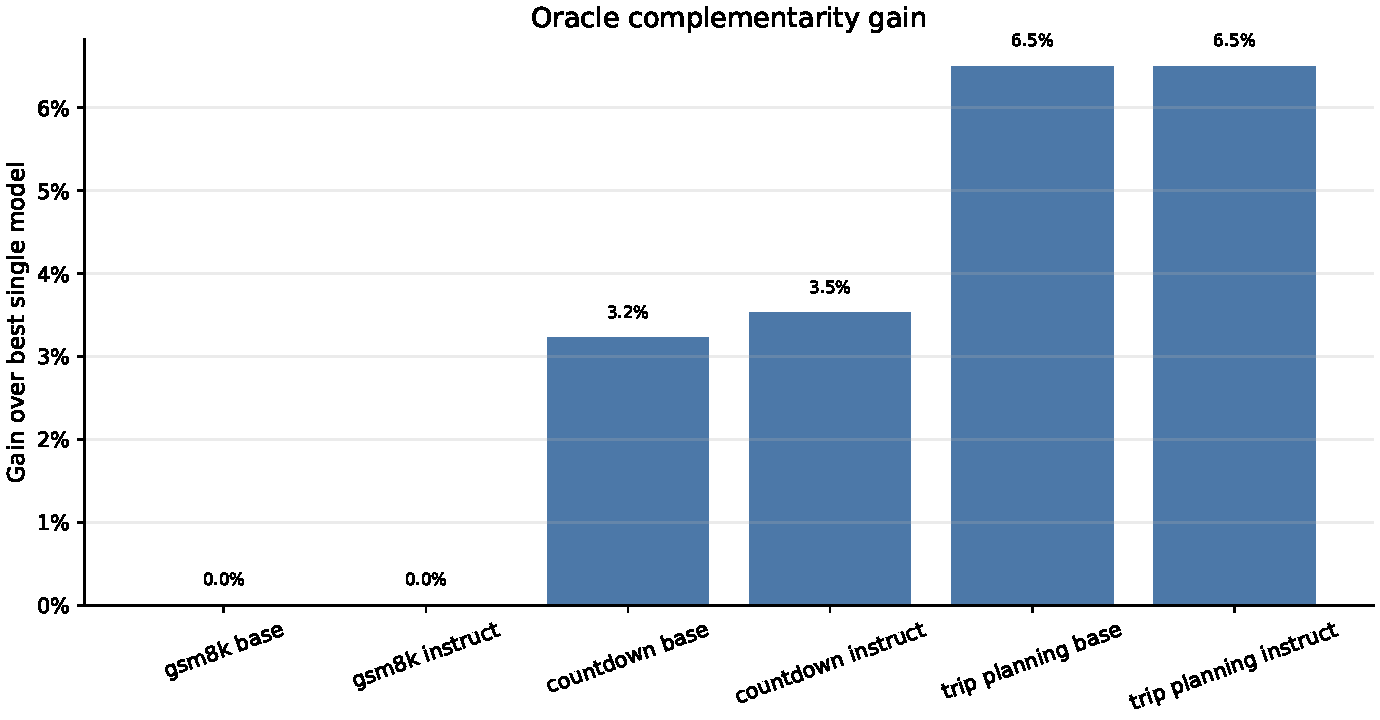
\includegraphics[width=0.84\textwidth]{images/oracle_ensemble_gain.pdf}
\caption{Oracle complementarity gain over the best single model. GSM8K is saturated, but both planning benchmarks show measurable paradigm-level union gains.}
\label{fig:oracle-gain}
\end{figure}

\begin{table}[!htbp]
\centering
\caption{Oracle complementarity from existing samples. Accuracies are percentages of questions solved by at least one sample.}
\label{tab:oracle-summary}
\footnotesize
\setlength{\tabcolsep}{4pt}
\scriptsize
\begin{tabularx}{\textwidth}{L{2.2cm}YYcc}
\toprule
\textbf{Condition} & \textbf{Best single} & \textbf{Best dLLM + AR union} & \textbf{All-model union} & \textbf{Gain} \\
\midrule
GSM8K base & Qwen $100.00$ & LLaDA + Qwen $100.00$ & $100.00$ & $0.00$ \\
GSM8K instruct & Qwen $100.00$ & LLaDA + Qwen $100.00$ & $100.00$ & $0.00$ \\
Countdown base & Qwen $51.31$ & Dream + Qwen $54.54$ & $60.89$ & $3.23$ \\
Countdown instruct & Llama $46.17$ & Dream + Llama $49.70$ & $50.50$ & $3.53$ \\
Trip Planning base & Llama $25.50$ & Dream + Llama $32.00$ & $35.50$ & $6.50$ \\
Trip Planning instruct & Llama $21.00$ & Dream + Llama $27.50$ & $29.00$ & $6.50$ \\
\bottomrule
\end{tabularx}
\end{table}

The oracle analysis makes the complementarity claim concrete. On Countdown base, the best single model solves $509$ of $992$ questions, but a Dream$+$Qwen oracle union solves $541$ and the full four-model union solves $604$. Trip Planning is even more striking relative to its scale: the best single model solves $51$ of $200$ base questions, while Dream$+$Llama solves $64$ and the full four-model union solves $71$. These numbers are upper bounds because no practical selector is implemented, but they show that the correlation results are not merely statistical decoration --- the gap between best-single-model and best-paradigm-union is large enough on planning benchmarks to motivate a follow-up project on selective routing or combiner training.
